%% Supporting Information for the Water Resources Research submission.
%% Built by scripts/223_wrr_build.py alongside the article. AGU numbers
%% supporting items S1, S2, ...; that renumbering is set below.

\documentclass[draft]{agujournal2025}

\usepackage{booktabs}
\usepackage{amsmath}

\renewcommand{\thefigure}{S\arabic{figure}}
\renewcommand{\thetable}{S\arabic{table}}
\renewcommand{\thesection}{S\arabic{section}}

\begin{document}

\journalname{Water Resources Research}

\title{Supporting Information for ``Measure missingness where the statistic
lives: a continuous screening law for gap-affected stream-temperature records''}

\authors{AUTHOR ONE\affil{1}}
\affiliation{1}{AFFILIATION PENDING AUTHOR CONFIRMATION}
\authoraddr{Corresponding author details pending author confirmation.}
\authorrunninghead{Ignored.}
\titlerunninghead{Ignored.}

\maketitle

\section*{Contents of this file}

\begin{enumerate}
  \item Text S1 to S6
  \item Figures S1 to S5
  \item Table S1
\end{enumerate}

\section*{Introduction}

This supporting information records what belongs to the record rather than to
the argument: data provenance, protocol history, the predictions declared for
this round that were not met, the runs that were discarded and why, and the
reproduction path. Nothing here is required to follow the article.

\section{Data sources}

Daily water-temperature series were assembled from nine public providers
(Table~\ref{tab:si-providers}). All are open archives; none required a data-use
agreement.

\begin{table}
\caption{Providers and their role in the study.}
\label{tab:si-providers}
\centering
\begin{tabular}{lll}
\hline
provider & country & role \\
\hline
ARSO & Slovenia & development \\
CHMI & Czechia & development \\
FOEN & Switzerland & development and reserved \\
GKD Bayern & Germany (Bavaria) & development and reserved \\
LUBW & Germany (Baden-W\"urttemberg) & development and reserved \\
NVE & Norway & development and reserved \\
Rijkswaterstaat & Netherlands & development and reserved \\
SYKE & Finland & development and reserved \\
USGS & United States & development and reserved \\
\hline
\end{tabular}
\end{table}

Station coordinates were assembled for all 457 stations: from the providers'
own catalogues already held in the repository for FOEN, CHMI, SYKE, LUBW, GKD
Bayern, NVE and Rijkswaterstaat and for nine USGS gauges; from the USGS NWIS
site service for the remaining 195 United States gauges; and from ARSO's public
station feed for all 47 Slovenian stations. Every row of the coordinate table in
the repository records its source.

Daily 2\,m air temperature is NASA POWER (MERRA-2), 1 January 1981 to 31 August
2026, one point per station at the product's native resolution: 16{,}679 days
for each of the 457 stations. An earlier version of this study used a much
smaller forcing table covering 2.3\% of development cases; both are retained and
Section 5.7 of the article compares them.

Basin characteristics for the United States subset are GAGES-II, joined on the
eight-digit gauge identifier and matching 140 of 204 eligible stations.

\section{Quality control and the definition of a network}

A \emph{network} is a provider's group of stations on a common river system,
which is the unit at which donor stations are available to one another. Networks
are the clustering unit for every interval in the article, because station-years
within a network share weather, regulation and instrumentation.

Waterbody class was assigned per network from the provider's own naming and an
explicit map; seas, lakes, canals, estuaries and deltas are listed and excluded
rather than averaged into a river result. Reference series are never imputed: a
calendar year with any missing day contributes no truth. Stations with fewer
than four fully observed calendar years are excluded, because the
leave-one-year-out estimator protocol requires them. The resulting denominator,
with every exclusion and its count, is in the repository. The same stations
contribute 2422 station-years with at least 360 daily slots and at least one
missing day; those form the deployment panel of Section 5.10 of the article.

\section{Protocol history}

The study was pre-registered before the reserved networks were opened on
2026-09-23. Three aspects of that freeze were incomplete or wrong and are
recorded here rather than silently repaired.

\textbf{The incumbent's imputed limit was mis-stated.} An earlier version placed
the comparison at a thirteen-week (91-day) limit attributed to Johnson et al.
(2021). The source says twenty weeks. The analysis code now uses 140 days and
every artifact that used the old value was re-run; Section 5.6 of the article
reports the corrected operating point. The direction of the error flattered the
incumbent at that point, so correcting it reduces the screen's advantage there
from 6.2 to 4.4 percentage points.

\textbf{The weighting between outage arms was not declared.} The case set mixes
an empirical arm, drawn from the outage geometry the same networks experience,
with a stratified arm built to span the decision space. Their base rates differ
by an order of magnitude. The pre-registered test was run on the pooled set, as
declared; Section 5.9 reports the decomposition and states that the declared
effect is not met on the empirical arm alone.

\textbf{The natural scale of the peak has two values.} Computed over the full
eligible roster it is 1.06\,$^{\circ}$C; recomputed inside the development case
table it is 1.08\,$^{\circ}$C. The primary tolerance is 0.50\,$^{\circ}$C
throughout except in cross-metric comparisons, where each endpoint's scale is
recomputed on the same footing. The tolerance sweep shows the axis ordering is
unchanged between 0.25 and 1.0 standard deviations.

\section{Predictions that failed}

Three predictions were written down before the analyses that tested them and
were not met. All three are in the article; they are gathered here because a
reader looking for them should not have to hunt.

\begin{enumerate}
  \item \emph{The support-restricted advantage will decay monotonically in the
    support width.} It does not: it is a hump peaking at a 60-day support.
  \item \emph{The estimand's own support is the best conditioning set at every
    support width.} It is not: below 30 days a fixed 30-day window beats it.
  \item \emph{For the sine-fit phase, two hand-chosen transition windows will
    beat both peak-window overlap and outage length.} They beat peak overlap
    decisively and tie outage length.
\end{enumerate}

Failures 1 and 2 have one cause, which we then measured: the support's location
is itself uncertain, so the conditioning set has to be the support dilated by
that uncertainty. Failure 3 has a related cause: a hand-drawn window is a crude
approximation to an influence function that is spread over half the year.

A fourth statement was \emph{withdrawn} rather than falsified. An earlier version
framed the standing guidance as getting an ordering backwards. On the guidance's
own estimands it does not; Section 5.4 of the article reports that a completeness
threshold is the correct axis for the sine-fit mean and within 0.02 AUC of the
best for the phase.

\section{Runs that were discarded}

Two defects made specific artifacts unusable and both were repaired before the
reserved panel was opened: outage realizations were seeded from a process-salted
hash, so the case table could not be regenerated, and worker results were
concatenated in completion order, so the row order was not reproducible even
though the content was. A third defect affected the calibration rather than the
data: an additive, per-estimator conformal scheme under-covered, because
selecting the smallest of several bounds is a winner's curse that per-estimator
calibration cannot see. In all three cases the affected numbers were discarded
rather than reported alongside the repaired ones, and the pipeline was re-run in
full.

\section{Verification and reproduction}

\begin{itemize}
  \item The case table is byte-reproducible including row order, pinned by a
    test.
  \item The extended endpoint table regenerates the same 51{,}524 realizations
    from the same deterministic seeds, which is how its rows line up with the
    main case table; a test checks the alignment.
  \item No feature may read a day the outage hides; enforced in the feature
    constructor and pinned by a test.
  \item Every table cell and audited inline number in the article is re-derived
    from the artifacts by an audit script that the test suite runs.
  \item The schematic figures are generated from editable draw.io sources held
    in the repository; a test checks that each exported PDF is newer than its
    source.
\end{itemize}

Figure~\ref{fig:si-chain} lays the study out as a chain and labels each link with
the research question that establishes it, including the two links that earlier
versions of this work left open and this one closes.

\begin{figure}
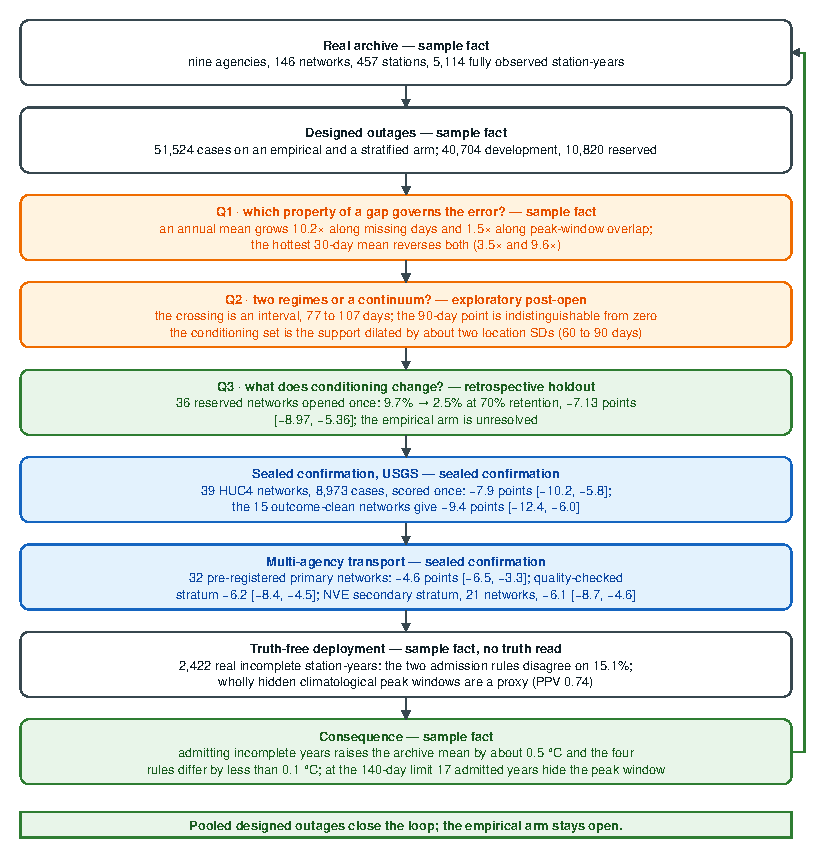
\includegraphics[width=\textwidth]{figures/f3_evidence_chain.pdf}
\caption{The evidence chain by research question. Every link is labelled with
the section that establishes it; the deployment and consequence links, drawn
open in earlier versions of this work, are closed here, and the consequence link
carries the finding that the regional aggregate barely moves.}
\label{fig:si-chain}
\end{figure}


\section{Supporting figures}

\begin{figure}[htbp]
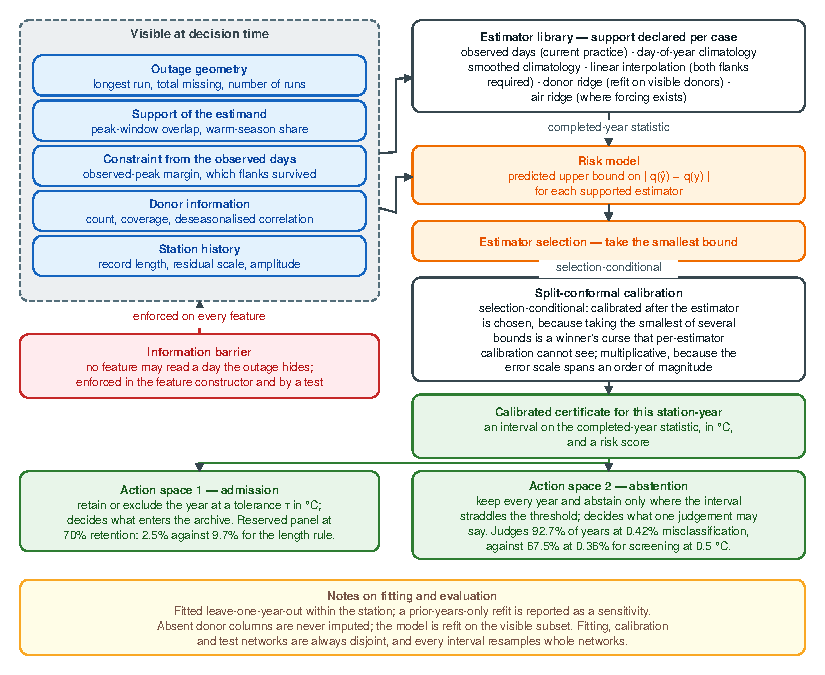
\includegraphics[width=\textwidth]{figures/f1_system_architecture.pdf}
\caption{The screening system in detail. Left: the features visible at decision time, under an information barrier that forbids any feature from reading a day the gap hides. Centre: the estimator library with per-case support, the risk model, estimator selection, and the selection-conditional multiplicative conformal calibration. Bottom: the two action spaces the same calibrated object supports.}
\label{fig:si-arch}
\end{figure}

\begin{figure}[htbp]
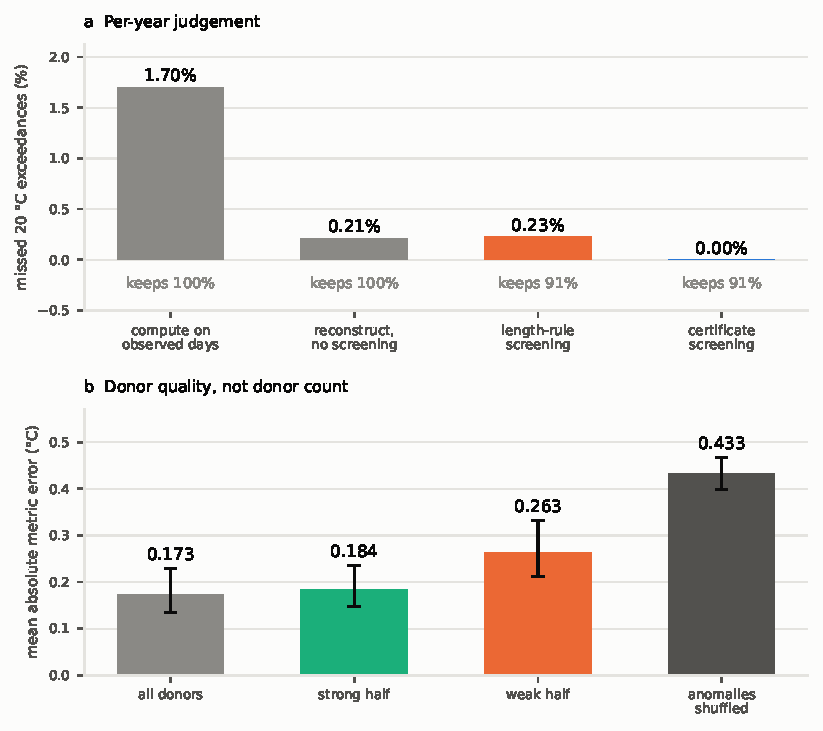
\includegraphics[width=\textwidth]{figures/fig4_consequence.pdf}
\caption{Multi-year trend error (a) and the donor controls (b). The panel averages eleven complete years per station, which is too short to resolve a decadal trend; the slope error is reported as a diagnostic of the reconstruction rather than as a trend estimate.}
\label{fig:si-cons}
\end{figure}

\begin{figure}[htbp]
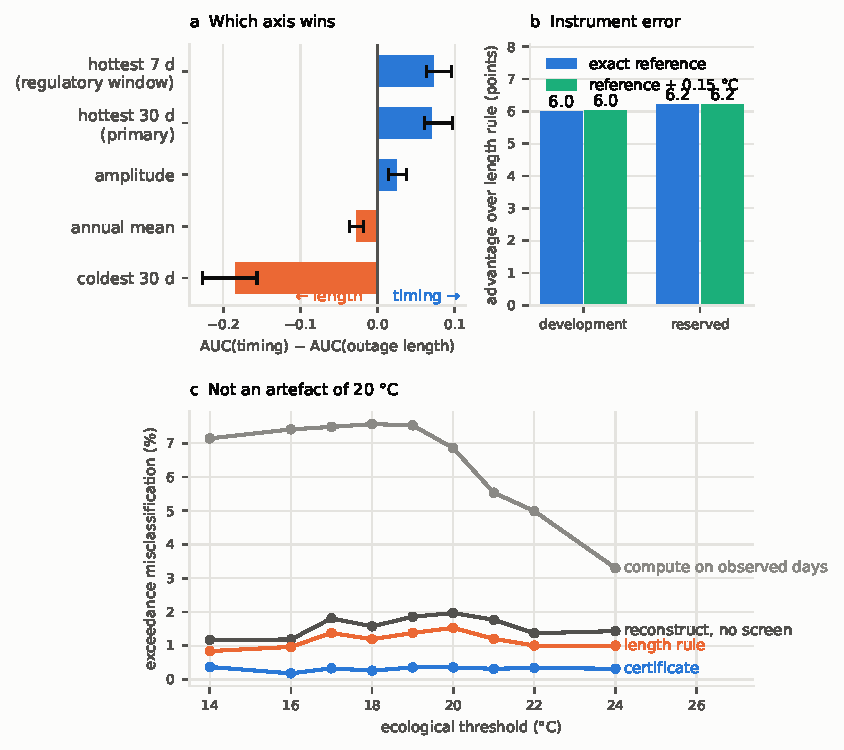
\includegraphics[width=\textwidth]{figures/fig5_robustness.pdf}
\caption{Network-clustered intervals on the axis contrasts (a), the reference-noise perturbation (b), and the exceedance-threshold sweep (c).}
\label{fig:si-robust}
\end{figure}

\begin{figure}[htbp]
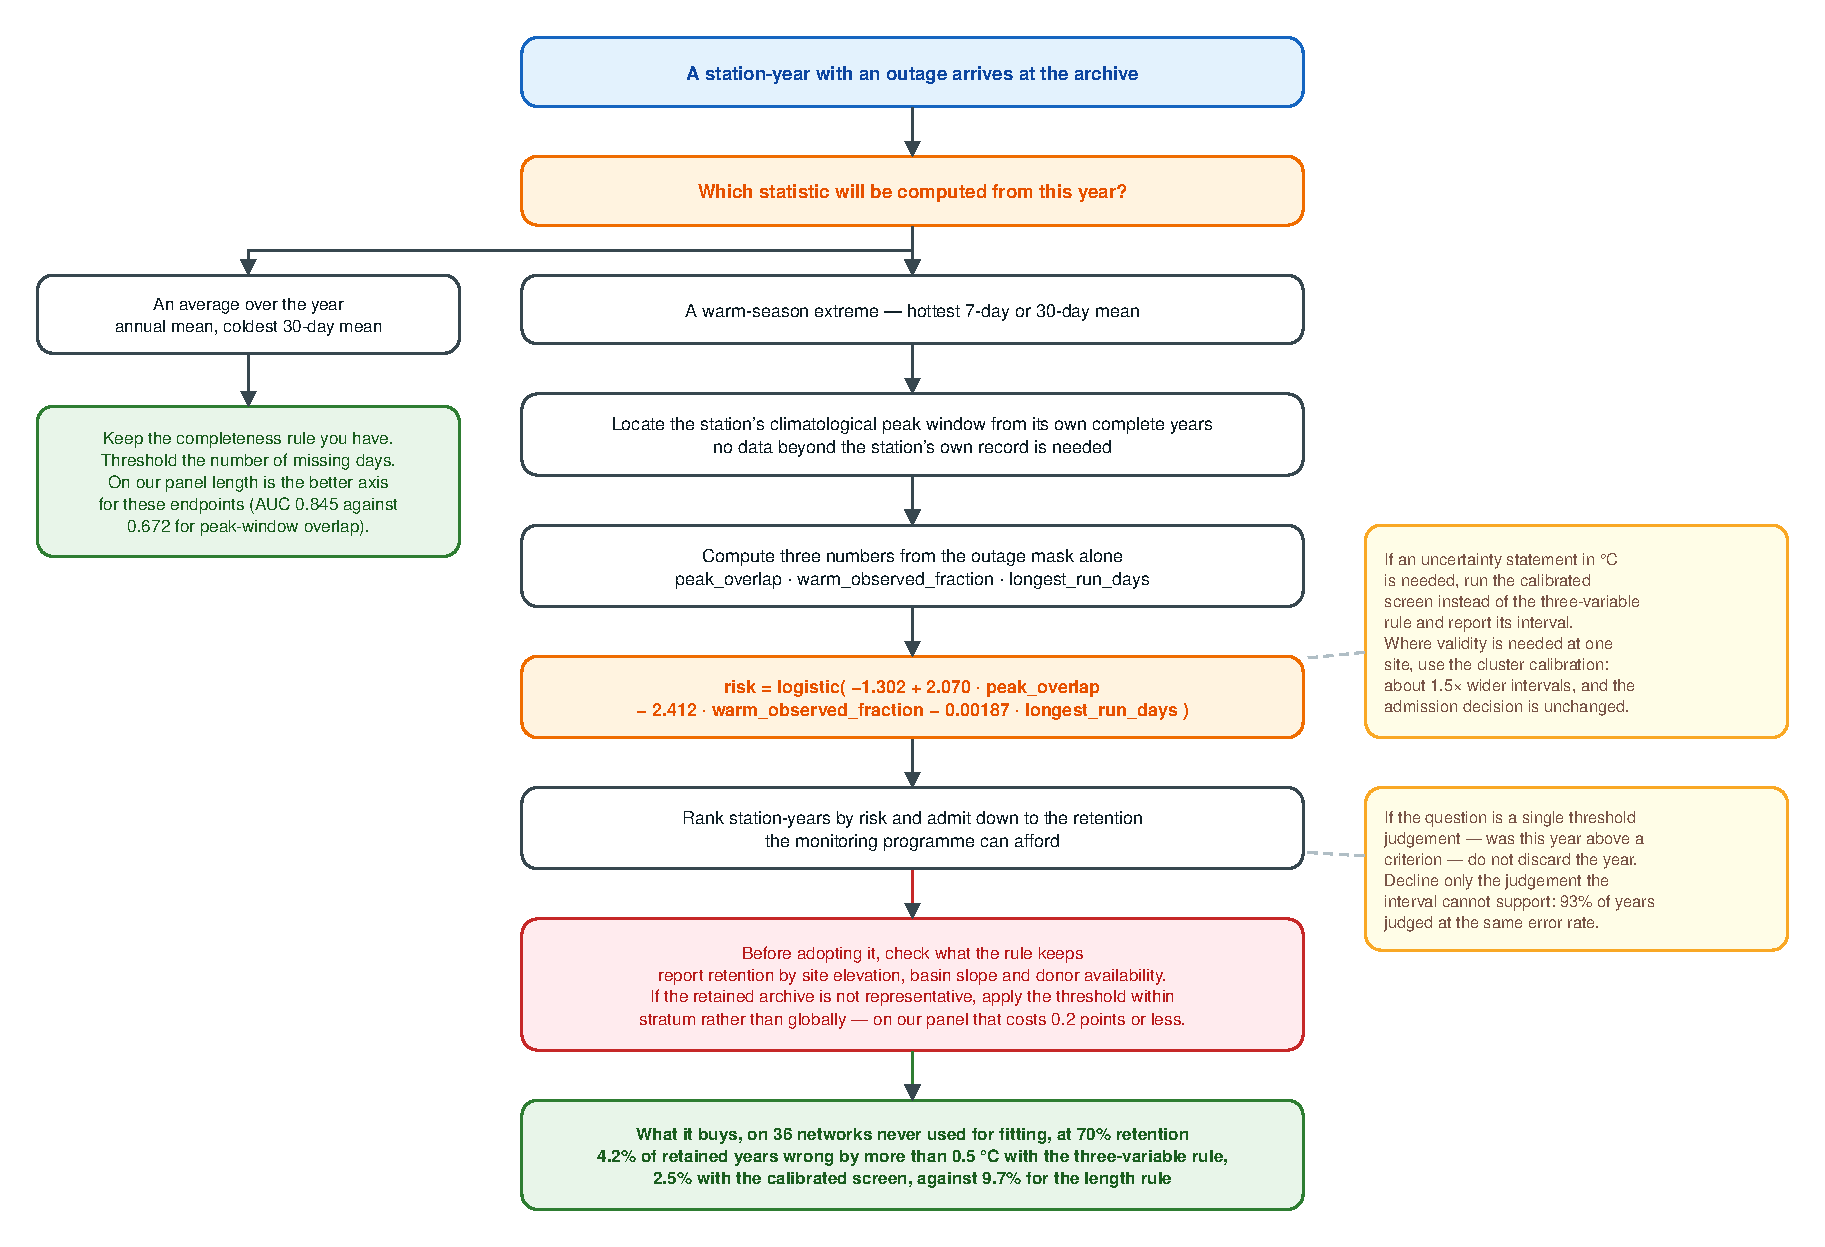
\includegraphics[width=\textwidth]{figures/f4_deployment_workflow.pdf}
\caption{What an agency does with the result: which endpoint, where the peak window comes from, the three numbers of the deployable rule, the representativeness guardrail, and what the substitution buys on networks never used for fitting.}
\label{fig:si-workflow}
\end{figure}

\end{document}
